\section{Metric Spaces}
\subsection{Definitions and Examples}

\begin{question}
    Can we think about convergence in a more general setting? Convergence seemed similar in our 3 settings.

    What do we really need?
\end{question} 
\begin{answer}
    We need a notion of distance.

    In $\mathbb{R}$: distance $x$ to $y$ is $|x-y|$. \\
    In $\mathbb{R}^2$: its $\norm{x - y}$. \\
    For functions: distance $f$ to $g$ is $\sup_{x \in X} |f(x) - g(x)|$ (where this exists, i.e. if $f - g$ bounded).

    The triangle inequality was often important (see the proof of uniqueness of limits).
\end{answer}

\begin{definition}[Metric]
    A $\vocab{metric}$ $d$ is a function $d : X^2 \to \mathbb{R}$ satisfying:
    \begin{itemize}
        \item $d(x, y) \geq 0$ for all $x, y \in X$ with equality iff $x = y$;
        \item $d(x, y) = d(y, x)$ for all $x, y \in X$.
        \item $d(x, z) \leq d(x, y) + d(y, z)$ for all $x, y, z \in X$.
    \end{itemize} 
\end{definition} 

\begin{definition}[Metric Space]
    A $\vocab{metric space}$ is a set $X$ endowed with a metric $d$.
\end{definition} 
We could also define a metric space as an ordered pair $(X, d)$.
If it is obvious what $d$ is, we sometimes write `The metric space $X$ \dots'.

\begin{example}
    $X = \mathbb{R}$, $d(x, y) = |x - y|$
    `The \underline{usual metric} on $\mathbb{R}$'.
\end{example} 

\begin{example}
    $X = \mathbb{R}^n$ with the \underline{Euclidean metric}, $d(x, y) = \norm{x - y} = \sqrt{\sum_{i=1}^{n} (x_i - y_i)^2}$.
\end{example} 

Uniform convergence of functions doesn't quite work: we want $d(f, g) = \sup |f - g|$ but this might not exist if $f - g$ is unbounded.
However, we can do something with appropriate sets of functions.

\begin{example} \label{exm:2.3}
    Let $Y \subset \mathbb{R}$.
    Take $X = B(Y) = \{f : Y \to \mathbb{R} \mid f \text{ bounded}\}$ with the \underline{uniform metric} $d(f, g) = \sup_{x \in Y} |f - g|$.

    Checking triangle inequality:
    \begin{proof}
        Let $f, g, h \in B(Y)$.
        Let $x \in Y$.
        Then \begin{align*}
            |f(x) - h(x)| &\leq |f(x) - g(x)| + |g(x) - h(x)| \\
            &\leq d(f, g) + d(g, h)
            \intertext{Taking $\sup$ over all $x \in Y$}
            d(f, h) \leq d(f, g) + d(g, h).
        \end{align*} 
    \end{proof} 
\end{example} 

\begin{definition}[Subspace]
    Suppose $(X, d)$ a metric space and $Y \subset X$.
    Then $d\mid_{Y^2}$ is a metric on $Y$.
    We say $Y$ with this metric is a \vocab{subspace} of $X$.
\end{definition} 

\begin{example}
    Subspaces of $\mathbb{R}$: any of $\mathbb{Q}, \mathbb{Z}, \mathbb{N}, [0, 1], \dots$ with the usual metric $d(x, y) = |x-y|$.
\end{example} 

\begin{example}
    Recall that a cts function on a closed bounded interval is bounded.
    Define $C([a, b]) = \{f:[a, b] \to \mathbb{R} \mid f \text{ cts}\}$.
    This is a subspace of $B([a, b])$, \cref{exm:2.3}.
    That is $C([a, b])$ is a metric space with the uniform metric $\mathcal{L}(f, g) = \sup_{x \in [a, b]} |f(x) - g(x)|$
\end{example} 

\begin{example}
    The empty metric space $X = \emptyset$ with the empty metric.
\end{example} 

Could maybe define different metrics on the same set:
\begin{example}
    The $\ell_1$ metric on $\mathbb{R}^n$: $d(x, y) = \sum_{i=1}^{n} |x_i - y_i|$.
\end{example} 

\begin{example}
    The $\ell_\infty$ metric on $\mathbb{R}^n$: $d(x, y) = \max_{i} |x_i - y_i|$.\footnote{Proof of triangle inequality similar to \cref{exm:2.3}}
\end{example} 

\begin{example}
    On $C([a, b])$ we can define the $L_1$ metric: $d(f, g) = \int_a^b |f-g|$.
\end{example} 

\begin{example}
    $X = \mathbb{C}$ with 
    \begin{align*}
        d(z, w) = \begin{cases}
            0 & z = w \\
            |z| + |w| & z \neq w.
        \end{cases}.
    \end{align*}

    First two conditions of a metric hold obviously, for triangle inequality we need $d(u, w) \leq d(u, v) + d(v, w)$.

    \begin{enumerate}
        \item If $u = w$, LHS = 0 \checkmark
        \item If $u = v$ or $v = w$ then LHS = RHS \checkmark
        \item If $u, v, w$ distinct:
        \begin{align*}
            LHS &= |u| + |w| \\
            RHS &= |u| + |w| + 2|v| \checkmark
        \end{align*} 
    \end{enumerate} 

    This metric is often called the British Rail metric or SNCF metric, you can think of it as for distinct points you have to travel through the origin.
    {\par 
\centering 
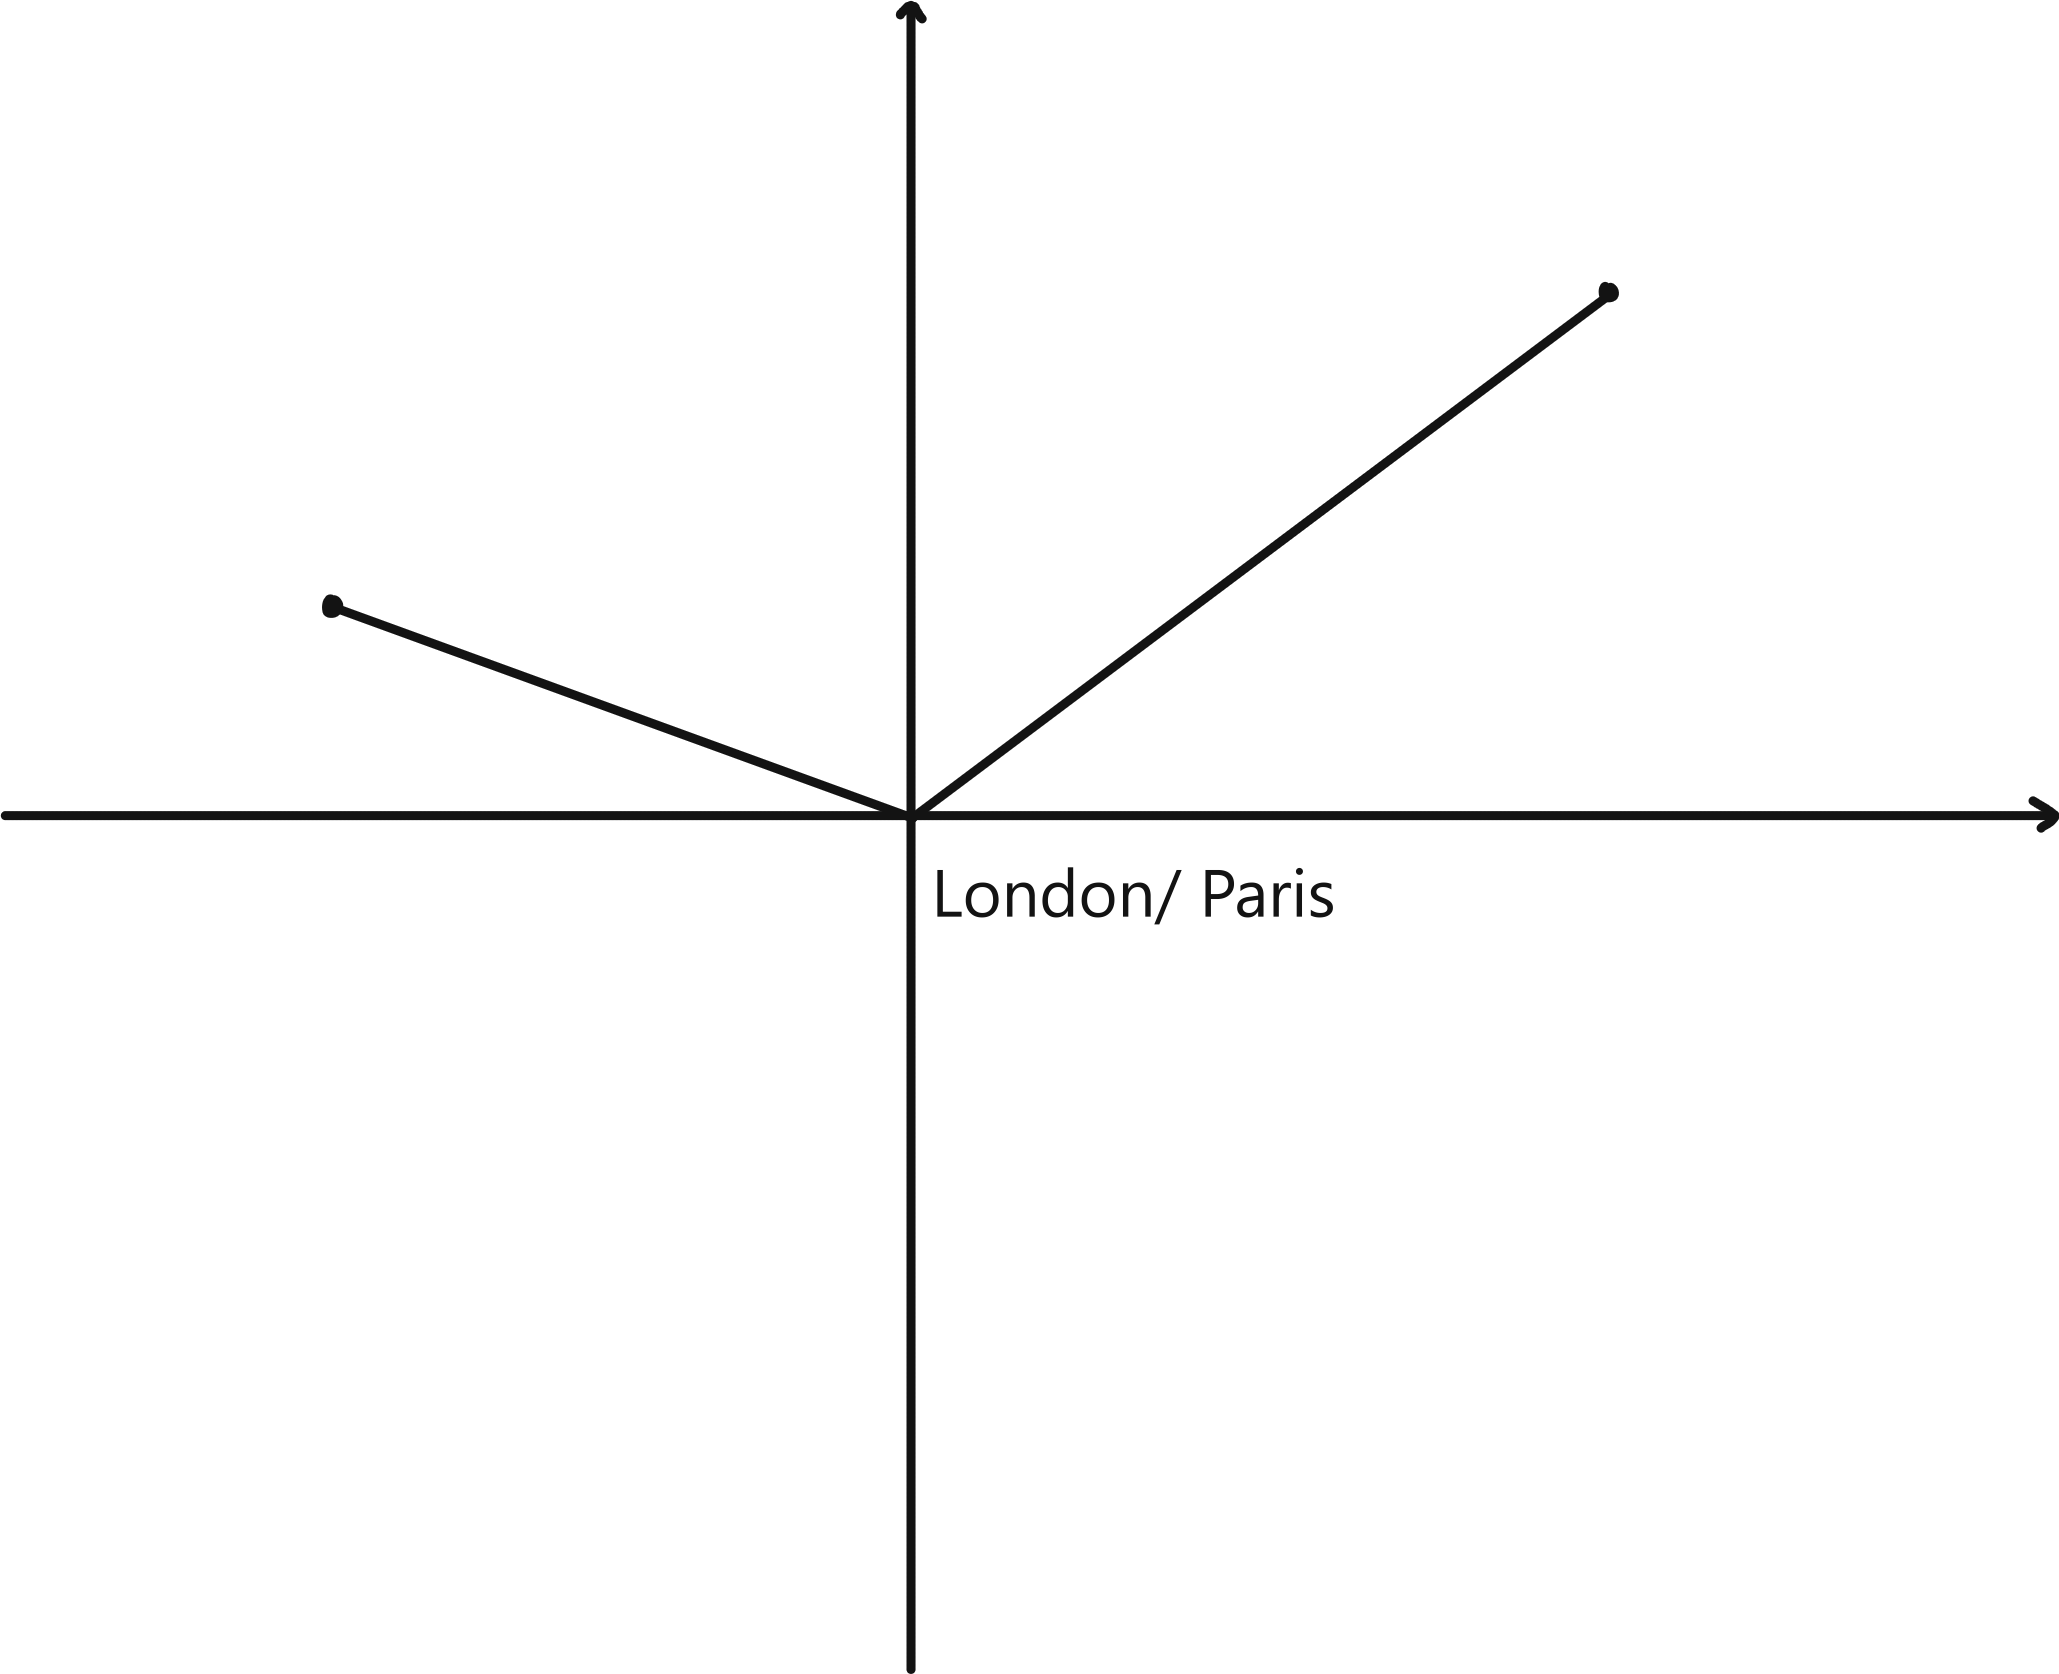
\includegraphics[height=5cm]{02-britishrail} 
    \par}
\end{example} 

\begin{example}[Discrete metric] \label{exm:discrete}
    Let $X$ be any set.
    Define a metric $d$ on $X$ by
    \begin{align*}
        d(x, y) = \begin{cases}
            0 & x = y \\
            1 & x \neq y.
        \end{cases} 
    \end{align*} 

    Easy to check this works.
    This is called the \underline{discrete metric} on $X$.
\end{example} 

\begin{example}[$p$-adic metric]
    Let $\mathbb{X} = \mathbb{Z}$.
    Let $p$ be a prime.
    The \vocab{$p$-adic metric} on $\mathbb{Z}$ is the metric $d$ defined by:
    \begin{align*}
        d(x, y) = \begin{cases}
            0 & x = y \\
            p^{-a} & \text{if $x \neq y$ and $x - y = p^a m$ with $p \nmid m$\footnote{$p^a$ is the largest $a$ s.t. $p^a \mid x - y$}.}
        \end{cases} 
    \end{align*} 
    `Two numbers are close if difference is divisible by a large power of $p$'.

    Only thing we need to check is triangle inequality
    \begin{proof}
        STP: $d(x, z) \leq d(x, y) + d(y, z)$
        \begin{enumerate}
            \item If $x = z$, LHS = 0 \checkmark
            \item If $x = y$ or $y = z$ then LHS = RHS \checkmark
        \end{enumerate} 

        So easy if any two of $x, y, z$ the same so assume $x, y, z$ all distinct.
        Let $x - y = p^a m$ and $y - z = p^b n$ where $p \nmid m, p \nmid n$ and wlog $a \leq b$.
        So $d(x, y) = p^{-a}$ and $d(y, z) = p^{-b}$.

        Now:
        \begin{align*}
            x - z &= (x - y) = (y - z) \\
            &= p^a m + p^b n \\
            &= p^a \underbracket{(m + p^{b - a} n)}_\text{integer} \text{ as $a \leq b$}.
        \end{align*} 
        So $p^a \mid x - z$ so $d(x, z) \leq p^{-a}$.
        But $d(x, y) + d(y, z) \geq d(x, y) = p^{-a}$.
    \end{proof} 
\end{example} 

\begin{definition}[Convergence]
    Let $(X, d)$ be a metric space, let $(x_n)$ be a sequence in $X$ and let $x \in X$.
    We say $(x_n)$ \vocab{converges} to $x$ and write `$x_n \to x$' or `$x_n \to x$ as $n \to \infty$' if
    \begin{align*}
        \forall \; \epsilon > 0 \ \exists \; N \ \forall \; n \geq N \ d(x_n, x) < \epsilon.
    \end{align*} 
\end{definition} 

Equivalently $x_n \to x$ iff $d(x_n, x) \to 0$ in $\mathbb{R}$.

\begin{proposition} \label{prp:15}
    Limits are unique.
    That is, if $(X, d)$ is a metric space, $(x_n)$ a sequence in $X$, $x, y \in X$ with $x_n \to x$ and $x_n \to y$ then $x = y$.
\end{proposition} 

\begin{proof}
    For each $n$, 
    \begin{align*}
        d(x, y) &\leq d(x, x_n) + d(x_n, y) \text{ by triangle inequality} \\
        &\leq d(x_n, x) + d(x_n, y) \text{ by symmetry} \\
        &\to 0 + 0 = 0 \text{ as $d(x_n, x), d(x_n, y) \to 0$}
    \end{align*} 
    So $d(x, y) \to 0$ as $n \to \infty$.
    But $d(x, y)$ is constant so $d(x, y) = 0$ so $x = y$. 
\end{proof} 

\begin{remark}
    This justifies talking about \underline{the} limit of a convergent sequence in a metric space, and writing $x = \lim_{n \to \infty} x_n$ if $x_n \to x$.
\end{remark} 

\begin{remark}[Remarks on definition of convergence in a metric space] \
    \begin{enumerate}
        \item Constant sequences obviously converge. More over, eventually constant sequences converge.
        \item Suppose $(X, d)$ is a metric space and $Y$ is a subspace of $X$.
        Suppose $(x_n)$ is a sequence in $Y$ which converges in $Y$ to $x$.
        Then also $(x_n)$ converges in $X$ to $x$.

        However, converse is false: e.g. in $\mathbb{R}$ with the usual metric then $\frac{1}{n} \to 0$ as $n \to \infty$.
        Consider the subspace $\mathbb{R} \setminus \{0\}$.
        Then $(\frac{1}{n})$ is a sequence in $\mathbb{R} \setminus \{0\}$ but it doesn't converge in $\mathbb{R} \setminus \{0\}$.
        (Why? Suppose $\frac{1}{n} \to x$ in $\mathbb{R} \setminus \{0\}$.
        Then also $\frac{1}{n} \to x$ in $\mathbb{R}$. 
        But $\frac{1}{n} \to 0$ in $\mathbb{R}$ so by uniqueness of limits $x = 0$. But $x \in \mathbb{R} \setminus \{0\}$ and $0 \notin \mathbb{R} \setminus \{0\}$ \Lightning.)
    \end{enumerate} 
\end{remark} 

\begin{example}
    Let $d$ be the Euclidean metric on $\mathbb{R}^n$.
    Exactly as in $\mathbb{R}^2$, we have $x_n \to x$ iff the sequence converges in each coordinate in the usual way in $\mathbb{R}$.

    What about other metrics on $\mathbb{R}^n$?
    E.g. let $d_\infty$ be the uniform metric: $d_\infty(x, y) = \max_i |x_i - y_i|$.
    Which sequences converge in $(\mathbb{R}^n, d_\infty)$?
    $d(x, y) = \sqrt{\sum_{i=1}^{n} (x_i - y_i)^2} \leq \sqrt{\sum_{i=1}^{n} d_\infty(x, y)^2}$ so $d(x,y) \leq \sqrt{n} d_\infty(x,y)$.
    But also $d_\infty(x, y) \leq d(x, y)$ as one of the terms in $d(x, y)$ is $d_\infty^2$.

    Now suppose $(x_n)$ is a sequence in $\mathbb{R}^n$.
    Then $d(x_n, x) \to 0 \iff d(x_n, x) \to 0$.
    So exactly same sequences converge in $(\mathbb{R}^n, d)$ and $(\mathbb{R}^n, d_\infty)$

    What about $\ell_1$ metric $d_1$?
    $d_1(x, y) = \sum_{i=1}^{n} |x_i - y_i|$.
    Similarly, $d_\infty(x, y) \leq d_1(x, y) \leq n d_\infty(x, y)$.
    So again, exactly the same sequences converge in $(\mathbb{R}^n, d_1)$.
\end{example} 

\begin{example}
    Let $X = C([0, 1]) = \{f:[0, 1] \to \mathbb{R} \mid f \text{ continuous}\}$.
    Let $d_\infty$ be the uniform metric on $X$: $d_\infty(f, g) = \sup_{x \in [0, 1]} |f(x) - g(x)|$.
    \begin{align*}
        f_n \to f \text{ in } (X, d_\infty) &\iff d_\infty(f_n, f) \to 0 \\
        &\iff \sup_{x \in [0, 1]} |f_n(x) - f(x)| \to 0 \\
        &\iff f_n \to f \text{ uniformly.}
    \end{align*} 

    We also have $L_1$-metric $d_1$ on $X$: $d_1(f, g) = \int_0^1 |f - g|$.
    Now $d_1(f, g) = \int_0^1 |f-g| \leq \int_0^1 d_\infty(f, g) = d_\infty(f, g)$.
    So similarly to previous example,
    \begin{align*}
        f_n \to f \text{ in } (X, d_\infty) \implies f_n \to f \text{ in } (X, d_1).
    \end{align*} 
    But converse does not hold, i.e. we can find a sequence $(f_n)$ in X s.t. $f_n \to 0$ in $d_1$-metric but $f_n$ doesn't converge in $d_\infty$-metric, i.e. $\int_0^1 |f_n| \to 0$ as $n \to \infty$ but $(f_n)$ does not converge uniformly.
    {\par
    \centering 
    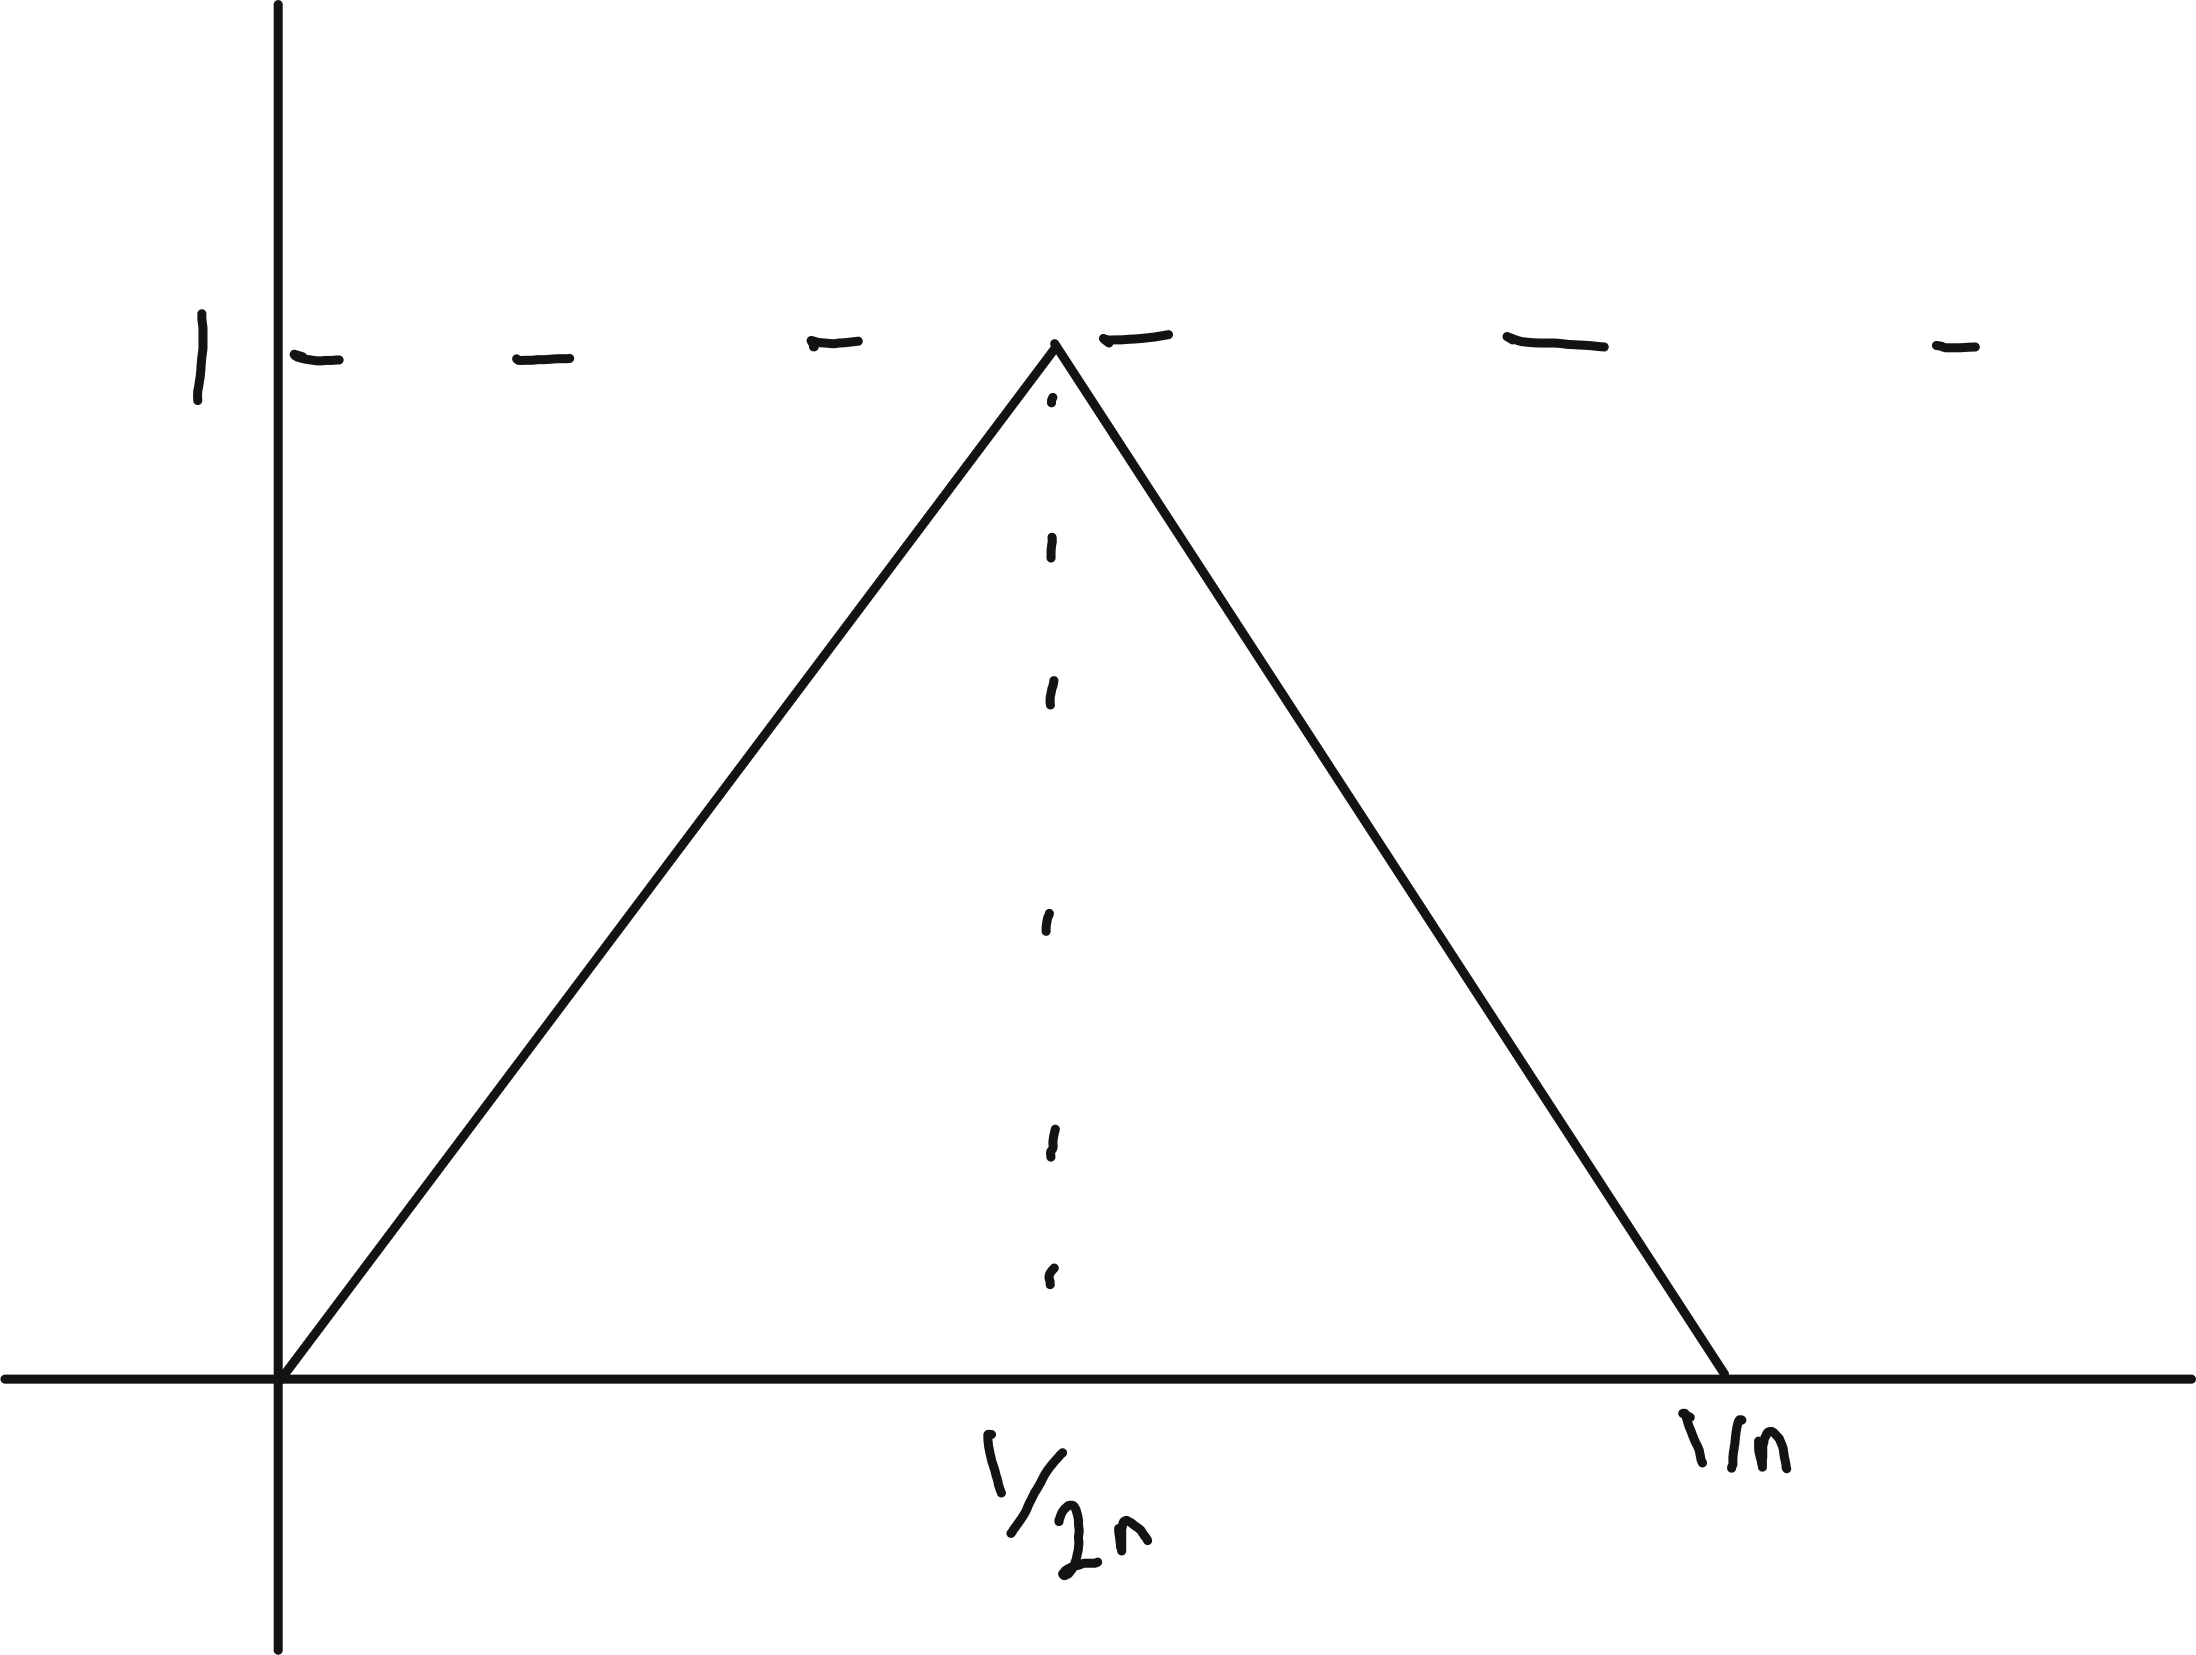
\includegraphics[height=5cm]{02-exm2.14} 
    \par}
    \begin{align*}
        f_n(x) = \begin{cases}
            2nx & x \leq \frac{1}{2n} \\
            2n (\frac{1}{n} - x) & \frac{1}{2n} < x \leq \frac{1}{n} \\
            0 & x > \frac{1}{n}.
        \end{cases} 
    \end{align*}
    Then $d_1(f_n, 0) = \frac{1}{2} \times \frac{1}{n} \times 1 = \frac{1}{2n} \to 0$.
    So in $(X, d_1)$ we have $f_n \to 0$.
    But $f_n$ does not converge uniformly: indeed, $f_n \to 0$ pointwise; if we have uniform convergence then uniform limit is the same as pointwise limit; but $\forall \; n \ f_n(\frac{1}{2n}) = 1$ so $f_n \not\to 0$ uniformly.
\end{example} 

\begin{example}
    Let $(X, d)$ be a discrete metric space; $d(x, y) = \begin{cases}
        0 & x = y \\
        1 & x \neq y
    \end{cases}$.
    When do we have $x_n \to x$ if $(X, d)$?

    Suppose $x_n \to x$, i.e. $\forall \; \epsilon > 0 \ \exists \; N \ \forall \; n \geq N \ d(x_n, x) < \epsilon$.
    Setting $\epsilon = 1$ in this, we can find $N$ s.t. $\forall \; n \geq N \ d(x_n, x) < 1$, i.e. $\forall \; n \geq N \ d(x_n, x) = 0$ i.e. $\forall \; n \geq N \ x_n = x$.
    Thus $(x_n)$ is eventually constant. \\
    But we know in \underline{any} metric space, eventually constant sequences converge.

    So in this space, $(x_n)$ converges iff $(x_n)$ eventually constant.
\end{example} 

\begin{definition}[Continuity]
    Let $(X, d)$ and $(Y, e)$ be metric spaces and let $f : X \to Y$.
    \begin{enumerate}
        \item Let $a \in X$ and $b \in Y$.
        We say $f(x) \to b$ as $x \to a$ if $\forall \; \epsilon > 0 \ \exists \; \delta > 0 \ \forall \; x \in X \ 0 < d(x, a) < \delta \implies e(f(x), b) < \epsilon$. \label{def:con1}
        \item Let $a \in X$.
        We say $f$ is \vocab{continuous} at $a$ if $f(x) \to f(a)$ as $x \to a$. \\
        That is: $\forall \; \epsilon > 0 \ \exists \; \delta > 0 \ \forall \; x \in X \ d(x, a) < \delta \implies e(f(x), f(a)) < \epsilon$.
        \item If $\forall \; a \in X$ $f$ is continuous at $a$ we say $f$ is a \vocab{continuous} function or simply $f$ is \vocab{continuous}.
        \item We say $f$ is \vocab{uniformly continuous} if $\forall \; \epsilon > 0 \ \exists \; \delta > 0 \ \forall \; x,y \in X \ d(x, y) < \delta \implies e(f(x), f(y)) < \epsilon$
        \item Suppose $W \subset X$.
        We say $f$ is \vocab{continuous on $W$} (respectively \vocab{uniformly continuous on $W$}) if the function $f\mid_W$ is continuous (resp. uniformly continuous), as a function from $W \to Y$ where we are now thinking of $W$ as a subspace of $X$. \label{def:con5}
    \end{enumerate} 
\end{definition} 

% \begin{definition}[Uniform continuity]
%     We say $f$ is \vocab{uniformly continuous} if $\forall \; \epsilon > 0 \ \exists \; \delta > 0 \ \forall \; x,y \in X \ d(x, y) < \delta \implies e(f(x), f(y)) < \epsilon$
% \end{definition} 

\begin{remark}
    \begin{enumerate}
        \item Don't have a nice rephrasing of \cref{def:con1} in terms of similar concepts in the reals.
        We would want to write `$e(f(x), b) \to 0$ as $d(x, a) \to 0$'.
        But this is meaningless, we haven't defined such a concept in the reals.
        \item \Cref{def:con1} says nothing about what happens at the point $a$ itself. 
        E.g. let $f : \mathbb{R} \to \mathbb{R}, f(x) = \begin{cases}
            1 & x = 0 \\
            0 & x \neq 0
        \end{cases}$.
        Then $f(x) \to 0$ as $x \to 0$ (but $f(0) \neq 0$ so $f$ is not continuous at $0$). \\
        If we have $f$ cts then $d(x, a) = 0 \implies x = a \implies f(x) = f(a) \implies e(f(x), f(a)) = 0$.
        So we can drop the `$0 <$' from definition of continuity.
        \item We can rewrite \cref{def:con5}: $f$ is continuous on $W$ iff $f\mid_W$ is a continuous function $f\mid_W : W \to Y$ thinking of $W$ as a subspace of $X$.
        That is: $\forall \; a \in W \ \forall \; \epsilon > 0 \ \exists \; \delta > 0 \ \forall \; x \in X \ d(x, a) < \delta \implies e(f(x), f(a)) < \epsilon$.
        In particular, note the subtlety that this \underline{only} mentions points of $W$.
        So under this definition, e.g. $f : \mathbb{R} \to \mathbb{R}, f(x) = \begin{cases}
            1 & x \in [0, 1] \\
            0 & x \notin [0, 1]
        \end{cases}$ then $f\mid_{[0, 1]}$ is cts.
        But $f$ is not cts at points $0, 1$.
    \end{enumerate} 
\end{remark} 

\begin{proposition} \label{prp:16}
    Let $(X, d), (Y, e)$ be metric spaces, $f : X \to Y$ and $a \in X$.
    Then $f$ is continuous at $a$ iff whenever $(x_n)$ is a sequence in $X$ with $x_n \to a$ then $f(x_n) \to f(a)$.
\end{proposition} 

\begin{proof}
    ($\implies$): Suppose $f$ is cts at $a$.
    Let $(x_n)$ be a sequence in $X$ with $x_n \to a$.
    Let $\epsilon > 0$.
    As $f$ cts at $a$ we can find $\delta > 0$ s.t. $\forall \; x \in X$ s.t. $d(x, a) < \delta \implies e(f(x), f(a)) < \epsilon$.
    As $x_n \to x$ we can find $N$ s.t. $n \geq N \implies d(x_n, a) < \delta$.
    Let $n \geq N$ then $d(x_n, a) < \delta$ so $e(f(x_n), f(a)) < \epsilon$.
    Hence $f(x_n) \to f(a)$.

    ($\Longleftarrow$): Suppose $f$ is not cts at $a$.
    Then there is some $\epsilon > 0$ s.t. $\forall \; \delta > 0 \ \exists \; x \in X$ with $d(x, a) < \delta$ but $e(f(x), f(a)) \geq \epsilon$.
    Now take $\delta = \frac{1}{n}$ we obtain a sequence $(x_n)$ with, for each $n$ $d(x_n, a) < \frac{1}{n}$ but $e(f(x_n), f(a)) > \epsilon$.
    Hence $x_n \to a$ but $f(x_n) \not\to f(a)$.
\end{proof} 

\begin{proposition} \label{prp:17}
    Let $(W, c), (X, d), (Y, e)$ be metric spaces, left $f: W \to X$, let $g: X \to Y$ and let $a \in W$.
    Suppose $f$ is cts at $a$ and $g$ is cts at $f(a)$.
    Then $g \circ f$ is cts at $a$.
\end{proposition} 

\begin{proof}
    Let $(x_n)$ be a sequence in $W$ with $x_n \to a$.
    Then by \cref{prp:16}, $f(x_n) \to f(a)$ and so also $g(f(x_n)) \to g(f(a))$.
    So by \cref{prp:16} $g \circ f$ cts at a. 

    What?airsntaeirsnt
\end{proof} 

\begin{example} \label{exm:con1}
    In $\mathbb{R} \to \mathbb{R}$ with the usual metric, this is the same definition as when we defined continuity directly for $\mathbb{R}$ only.
    So we already have lots of cts fcns $\mathbb{R} \to \mathbb{R}$: polynomials, $\sin$, $e^x$, \dots
\end{example} 

\begin{example}
    Constant functions are continuous.
    Also if $X$ is any metric space and $f: X \to X$ by $f(x) = x$ for all $x \in X$ (the \underline{indentity function}) then that is continuous.
\end{example} 

\begin{example}[Projection Maps]
    Consider $\mathbb{R}^n$ with the usual metric and $\mathbb{R}$ with the usual metric.
    The \vocab{projection maps} $\pi_i: \mathbb{R}^n \to \mathbb{R}$ given by $\pi_i(x) = x_i$ are continuous. 
    
    (Why? We've seen convergence in $\mathbb{R}^n$ of sequences is the same as convergence in each coordinate. 
    Let's denote a sequence in $\mathbb{R}^n$ by $(x^{(m)})_{m \geq 1}$. So e.g. $x^{(3)}_5$ is the $5$th coord of the $3$rd term.
    We know $x^{(m)} \to x$ iff for each $i$ $x_i^{(m)} \to x_i$, i.e. for each $i$ $\pi_i(x^{(m)}) \to \pi_i(x)$.
    Then we can use \cref{prp:16})

    Similarly, suppose $f_1, \dots, f_n: \mathbb{R} \to \mathbb{R}$
    Let $f: \mathbb{R} \to \mathbb{R}^n$ defined by $f(x) = (f_1(x), \dots, f_n(x))$.
    Then $f$ is cts at a point iff all of $f_1, \dots, f_n$ are.
    Using these facts \cref{exm:con1} and \cref{prp:17}, we have many cts fcns $\mathbb{R}^n \to \mathbb{R}^m$.
    E.g. $f: \mathbb{R}^3 \to \mathbb{R}^2, f(x, y, z) = (e^{-x} \sin y, 2x \cos z)$ is cts. (Why? write $w = (x, y, z) \in \mathbb{R}^3$, we have $f_1(w) = e^{-\pi_1(w)} \sin \pi_2(w)$ and $f_2(w) = 2 \pi_1(w) \cos \pi_3(w)$.
    So $f_1, f_2$ cts so $f$ cts.)
\end{example} 

\begin{example}
    Recall that if we have the Euclidean metric, the $l_1$ or $l_\infty$ metric on $\mathbb{R}^n$ then the convergent sequences are the same.
    So by \cref{prp:16}, the ctf fcns $X \to \mathbb{R}^n$ or from $\mathbb{R}^n \to Y$ are the same with each of these three metrics.
\end{example} 

\begin{example}
    Let $(x, d)$ be the discrete metric space, \cref{exm:discrete}, and let $(Y, e)$ be any metric space.
    Which functions $f : X \to Y$ are cts?
    Suppose $a \in X$ and $(x_n)$ a sequence in $X$ with $x_n \to a$.
    Then $(x_n)$ is eventually constant, i.e. for sufficiently large $n$ $x_n = a$ and so $f(x_n) = f(a)$.
    So $f(x_n) \to f(a)$.

    Hence \underline{every} function on a discrete metric space is cts.
\end{example} 

\subsection{Completeness}
\begin{question}
    In \cref{sec:1} we saw a version of GPC held in each of the three examples we considered. 
    Does GPC hold in a general metric space?
\end{question} 

\begin{definition}[Cauchy Sequences]
    Let $(X, d)$ be a metric space and let $(x_n)$ be a sequence in $X$.
    We say $(x_n)$ is \vocab{Cauchy} if $\forall \; \epsilon > 0 \ \exists \; N \ \forall \; m, n \geq N \ d(x_m, x_n) < \epsilon$.
\end{definition} 

\begin{theorem}
    $(x_n)$ convergent $\implies (x_n)$ Cauchy.
\end{theorem} 
\begin{proof}
    Left as an exercise.
\end{proof} 

But converse is not true in general.

\begin{example} \label{exm:rnot0}
    Let $X = \mathbb{R} \setminus \{0\}$ with the usual metric and $x_n = \frac{1}{n}$.
    We say previously that $(x_n)$ does not converge. \\
    Note that $X$ is a subspace of $\mathbb{R}$.
    In $\mathbb{R}$ $(x_n)$ is convergent $(x_n \to 0)$ so $(x_n)$ is Cauchy in $\mathbb{R}$ so $(x_n)$ is Cauchy in $X$.
\end{example} 

\begin{example}
    $\mathbb{Q}$ with the usual metric.
    Let $x_n$ be $\sqrt{2}$ to $n$ decimal places.
    This converges in $\mathbb{R}$ so is Cauchy in $\mathbb{Q}$ but clearly doesn't converge in $\mathbb{Q}$.
\end{example} 

\begin{definition}[Completeness]
    Let $(X, d)$ be a metric space.
    We say $X$ is \vocab{complete} if every Cauchy sequence in $X$ converges.
\end{definition} 

\begin{example}
    \Cref{exm:rnot0} says $\mathbb{R} \setminus \{0\}$ with the usual metric is not complete. \\
    Similarly $Q$ with usual metric is not complete.
\end{example} 

\begin{example}
    GPC says $\mathbb{R}$ with the usual metric is complete.
\end{example} 

\begin{example}
    GPC for $\mathbb{R}^n$ says $\mathbb{R}^n$ with Euclidean metric is complete.
\end{example} 

\begin{example} \label{exm:gpuc}
    GPUC, \cref{thm:7}, (almost) says if $X \subset \mathbb{R}$ and $B(X) = \{f : X \to \mathbb{R} \mid f \text{ is bounded}\}$ with the uniform norm then $B(X)$ is complete.
\end{example} 

\begin{proof}
    Let $(f_n)$ be a Cauchy sequence in $B(X)$.
    Then $(f_n)$ is uniformly Cauchy so by GPUC is uniformly convergent.
    That is $f_n \to f$ uniformly for some $f: X \to \mathbb{R}$.
    As $f_n \to f$ uniformly we know $f_n - f$ is bounded for $n$ suff. large.
    Take such an $n$, then $f_n - f$ and $f_n$ are bounded so $f = f_n - (f_n  - f)$ is bounded.
    That is, $f \in B(X)$.
    Finally, $f_n \to f$ uniformly and $d(f_n, f) \to 0$, i.e. $f_n \to f$ in $(B(X), d)$.
\end{proof} 

\begin{remark}
    In many ways, this is typical of a proof that a given space $(X, d)$ is complete:
    \begin{enumerate}
        \item Take $(x_n)$ Cauchy in $X$;
        \item Construct/ find a putative limit object $x$ where it seems $(x_n)$ converges to $x$ in some sense;
        \item Show $x \in X$,
        \item Show $x_n \to x$ in metric space $(X, d)$ i.e. that $d(x_n, x) \to 0$.
    \end{enumerate} 
    This is often tricky/ fiddly/ annoying/ repetitive/ boring.
    But we need to take care as for example, it's tempting to talk about $d(x_n, x)$ while doing (ii) or (iii); but makes no sense to write `$d(x_n, x)$' until we have completed (iii) as $d$ is only defined on $X^2$ (if $x \notin X$ then can't use $d$).
\end{remark} 

\begin{example}
    If $[a, b]$ is a closed interval then $C([a, b])$ with uniform norm $d$ is complete.
\end{example} 

\begin{proof}
    (i): Let $(f_n)$ be a Cauchy sequence in $C([a, b])$. \\
    (ii): We know $C([a, b])$ is a subspace of $B([a, b])$ with uniform metric.
    We know $B([a, b])$ is complete by \cref{exm:gpuc} and $(f_n)$ is a Cauchy sequence in $B([a, b])$ so in $B([a, b])$, $f_n \to f$ for some $f$. \\
    (iii) Each $f_n$ is cts and $f_n \to f$ uniformly so $f$ is cts, i.e. $f \in C([a, b])$. \\
    (iv) Finally, each $f_n \in C([a, b])$, $f \in C([a, b])$ and $f_n \to f$ uniformly so $d(f_n, f) \to 0$.
\end{proof} 

This generalises:
\begin{definition}[Closed Metric Space]
    Let $(X, d)$ be a metric space and $Y \subset X$.
    We say $Y$ is \vocab{closed} if whenever $(x_n)$ a sequence in $Y$ with $x_n \to x \in X$ then $x \in Y$.
\end{definition} 

\begin{proposition} \label{prp:18}
    A closed subset of a complete metric space is complete.
\end{proposition} 

\begin{remark}
    This \underline{does} make sense: if $Y \subset X$ then $Y$ is itself a metric space or a subspace of $X$ so we can say e.g. `$Y$ is complete' to mean the metric space $Y$ (as a subspace of $X$) is complete.

    We could do exactly the same with any other properties of metric spaces we define.
\end{remark} 

\begin{proof}
    Let $(X, d)$ be a metric space and $Y \subset X$ with $X$ complete and $Y$ closed.
    (i): Let $(x_n)$ be a Cauchy sequence in $Y$. \\
    (ii): Now $(x_n)$ is a Cauchy sequence in $X$ so by completeness $x_n \to x$ in $X$ for some $x \in X$. \\
    (iii) $Y \subset X$ is closed so $x \in Y$. \\
    (iv) Finally we now have each $x_n \in Y, x \in Y$ and $x_n \to x$ in $X$, so $d(x_n, x) \to 0$ so $x_n \to x$ in $Y$.
\end{proof} 

\begin{example}
    Define $\ell_1 = \{ (x_n)_{n \geq 1} \in \mathbb{R}^\mathbb{N} \mid \sum_{n=1}^{\infty} |x_n| \text{ converges} \}$.
    Define a metric $d$ on $\ell_1$ by $d((x_n), (y_n)) = \sum_{n=1}^{\infty} |x_n - y_n|$.

    Note we have $\sum |x_n|, \sum |y_n|$ converge as we are in $\ell_1$.
    For each $n$ $|x_n - y_n| \leq |x_n| + |y_n|$ so by comparison test $\sum |x_n - y_n|$ converges.
    So $d$ is well-defined.
    Easy to check $d$ is a metric on $\ell_1$.
    Then $(\ell_1, d)$ is complete.
\end{example} 

\begin{proof}
    (i): Let $(x^{(n)})_{n \geq 1}$ be a Cauchy sequence in $\ell_1$, so for each $n$ $(x^{(n)}_i)_{i \geq 1}$ is a sequence in $\mathbb{R}$ with $\sum_{i=1}^{\infty} |x_i^{(n)}|$ convergent. \\
    % (ii) For each $n$, $(x_i^{(n)})_{i \geq 1}$ is a Cauchy sequence in $\mathbb{R}$ since if $y, z \in \ell_1$ then $|y_i - z_i| \leq d(y, z)$.
    % But $\mathbb{R}$ is complete, so for each $n$ we 
    (ii) For each $i$, $(x_i^{(n)})_{n \geq 1}$ is a Cauchy sequence in $\mathbb{R}$, since if $y, z \in \ell_1$ then $|y_i - z_i| \leq d(y, z)$.
    But $\mathbb{R}$ is complete, so for each $i$ we can find $x_i \in \mathbb{R}$ s.t. $x_i^{(n)} \to x_i$ as $n \to \infty$. \\
    Let $x = (x_1, x_2, \dots) \in \mathbb{R}^\mathbb{N}$. \\
    (iii) We next show $x \in \ell_1$, i.e. that $\sum_{i=1}^{\infty} |x_i|$ converges.

    Given $y \in \ell_1$, define $\sigma(y) = \sum_{i=1}^{\infty} |y_i|$, i.e. $\sigma(y) = d(y, z)$ where $z$ is the constant zero sequence. \\
    We now have, for any $m, n$
    \begin{align*}
        \sigma(x^{(m)}) &= d(x^{(m)}, z) \\
        &\leq d(x^{(m)}, x^{(n)}) + d(x^{(n)}, z) \\
        &= d(x^{(m)}, x^{(n)}) + \sigma(x^{(n)}) 
    \end{align*} 
    So $\sigma(x^{(m)}) - \sigma(x^{(n)}) \leq d(x^{(m)}, x^{(n)})$.
    Similarly, for any $m, n$ $\sigma(x^{(n)}) - \sigma(x^{(m)}) \leq d(x^{(m)}, x^{(n)})$ and so $|\sigma(x^{(m)}) - \sigma(x^{(n)})| \leq d(x^{(m)}, x^{(n)})$.
    Hence $(\sigma(x^{(m)}))_{m \geq 1}$ is a Cauchy sequence in $\mathbb{R}$, and so by GPC converges, say $\sigma(x^{(m)}) \to K$ as $m \to \infty$.

    \begin{claim}
        For any $I \in \mathbb{N}$, $\sum_{i=1}^{I} |x_i| \leq K + 2$.
    \end{claim}
    
    \begin{proof}
        As $\sigma(x^{(n)}) \to K$ as $n \to \infty$ we can find $N_1$ s.t. $n \geq N_1 \implies \sum_{i=1}^{\infty} |x_i^{(n)}| \leq K + 1$.
        Also, $n \geq N_1 \implies \sum_{i=1}^{I} |x_i^{(n)}| \leq K + 1$ (as each term non-negative).

        Next, for each $i \in \{1, 2, \dots, I\}$ we have $x_i^{(n)} \to x_i$ as $n \to \infty$.
        So we can find $N_2$ s.t. $n \geq N_2 \implies \forall \; i \in \{1, \dots, I\} \ |x_i^{(n)} - x_i| < I\inv$.

        Now let $n = \max (N_1, N_2)$ then $\sum_{i=1}^{I} |x_i| \leq \sum_{i=1}^{I} |x_i^{(n)}| + \sum_{i=1}^{I} |x_i^{(n)} - x_i| \leq K + 1 + I (I\inv) = K + 2$.
    \end{proof} 

    Now the partial sums of $\sum |x_i|$ are increasing and bounded above so $\sum |x_i|$ converges.
    That is $x \in \ell_1$. 

    (iv) Finally, need to check $x^{(n)} \to x$ as $n \to \infty$ in $\ell_1$, i.e. that $d(x^{(n)}, x) \to 0$ as $n \to \infty$. \\
    We have, for all $n, I$:
    \begin{align*}
        d(x^{(n)}, x) &= \sum_{i=1}^{\infty} |x_i^{(n)} - x_i| &\\
        &\leq \sum_{i=1}^{I} |x_i^{(n)} - x_i| + \sum_{i=I+1}^{\infty} |x_i^{(n)}| + \sum_{i=I + 1}^{\infty} |x_i|.
    \end{align*}
    Let $\epsilon>0$.
    We know $\sum |x_i|$ convergent (as $x \in \ell_1$) so we can pick $I_1$ s.t. $\sum_{i=I_1+1}^{\infty} |x_i| < \epsilon$. \\
    As $(x^{(n)})$ is Cauchy, we can find $N_1$ s.t. $m, n \geq N_1 \implies d(x^{(m)}, x^{(n)}) < \epsilon$.
    As $\sum_i |x_i^{(N_1)}|$ converges, we can find $I_2$ s.t. $\sum_{i=I_2+1}^{\infty} |x_i^{(N_1)}| < \epsilon$.
    Then
    \begin{align*}
        n \geq N_1 \implies \sum_{i=1}^{\infty} |x_i^{(n)}| &\leq \sum_{i=I_2 + 1}^{\infty} |x_i^{(N_1)}| + \sum_{i=I_2 = 1}^{\infty} |x_i^{(n)} - x_i^{(N_1)}| \\
        &< \epsilon + d(x^{(n)}, x^{(N_1)}) \\
        &< 2\epsilon.
    \end{align*} 
    Let $I = \max(I_1, I_2)$.
    For each $i = 1, 2, \dots, I$ we have $|x_i^{(n)} - x_i| \to 0$ as $n \to \infty$, so $\sum_{i=1}^{I} |x_i^{(n)} - x_i| \to 0$ as $n \to \infty$.
    Hence we can find $N_2$ s.t $n \geq N_2 \implies \sum_{i=1}^{I} |x_i^{(n)} - x_i| < \epsilon$.
    Let $N = \max(N_1, N_2)$ and let $n \geq N$.
    Then \begin{align*}
        d(x^{(n)}, x) &\leq \sum_{i=1}^{I} |x_i^{(n)} - x_i| + \sum_{i=I+1}^{\infty} |x_i^{(n)}| + \sum_{i=I+1}^{\infty} |x_i| \\
        &\leq \sum_{i=1}^{I} |x_i^{(n)} - x_i| + \sum_{i=I_2 + 1}^\infty |x_i^{(n)}| + \sum_{i=I_1 + 1}^{\infty} |x_i| \\
        &< \epsilon + 2\epsilon + \epsilon = 4\epsilon  
    \end{align*} 
    Hence $d(x^{(n)}, x) \to 0$ as $n \to \infty$, i.e. $x^{(n)} \to x$ in $\ell_1$. \\
    Hence $\ell_1$ is complete.
\end{proof} 

Now we will move on to main theorem of completeness.

\begin{definition}[Contraction mapping]
    Let $(X, d)$ be a metric space and $f:X \to X$.
    We say $f$ is a \vocab{contraction} if $\exists \; \lambda \in [0, 1)$ s.t. $\forall \; x, y \in X \ d(f(x), f(y)) \leq \lambda d(x, y)$.
\end{definition} 

\begin{theorem}[The Contraction Mapping Theorem] \label{thm:19}
    Let $(X, d)$ be a complete, non-empty metric space and $f: X \to X$ a contraction.
    Then $f$ has a unique fixed point.
\end{theorem} 

\begin{proof}
    Let $\lambda \in [0, 1)$ satisfy $\forall \; x, y \in X \ d(f(x), f(y)) \leq \lambda d(x, y)$. \\
    Let $x_0 \in X$.
    Recursively define $x_n = f(x_{n - 1})$ for $n \geq 1$.
    Let $\Delta = d(x_0, x_1)$.
    Then, by induction $d(x_n, x_{n+1}) \leq \lambda^n \Delta$ for all $n$. \\
    Now suppose $N \leq m < n$.
    Then
    \begin{align*}
        d(x_m, x_n) &\leq \sum_{i=m}^{n-1} d(x_i, x_{i + 1}) \\
        &\leq \sum_{i=m}^{n-1} \lambda^i \Delta \\
        &\leq \sum_{i=N}^{\infty} \lambda^i \Delta \\
        &= \frac{\lambda^N \Delta}{1 - \lambda} \to 0 \text{ as $N \to \infty$}.
    \end{align*}
    So $\forall \; \epsilon > 0 \ \exists \; N \ \forall \; m, n \geq N \ d(x_m, x_n) < \epsilon$ (i.e. we take $N$ s.t. $\frac{\lambda^N \Delta}{1 - \lambda} < \epsilon$).
    Thus $(x_n)$ is Cauchy, so by completeness converges, say $x_n \to x \in X$.
    But also $x_n = f(x_{n-1}) \to f(x)$ as $f$ continuous\footnote{follows immediately from definition of contraction mapping (e.g. let $\delta = \epsilon$ in definition of continuity).}.
    So by uniqueness of limits, $f(x) = x$.

    Suppose also $f(y) = y$ for some $y \in X$.
    Then $d(x, y) = d(f(x), f(y)) \leq \lambda d(x, y)$ with $\lambda < 1$.
    So $d(x, y) = 0$ so $x = y$.
\end{proof} 

\begin{remark} \
    \begin{enumerate}
        \item Why is $f$ cts? We have, for all $x, y \in X$ $d(f(x), f(y)) \leq d(x, y)$.
        So $\forall \; \epsilon > 0$, $d(x, y) < \epsilon \implies d(f(x), f(y)) < \epsilon$.
        (Indeed, this shows $f$ is uniformly continuous.)
        \item We have proved more than claimed.
        Not only does $f$ have a unique fixed point, but starting from \underline{any} point of the space and repeatedly apply $f$ then the resulting sequence converges to the fixed point.
        In fact, the speed of convergence is exponential.
    \end{enumerate} 
\end{remark} 

\begin{example}[Application]
    Suppose we want to numerically approximate the solution to $\cos x = x$.
    Any root must lie in $[-1, 1]$.
    Consider metric space $X = [-1, 1]$ with usual metric.
    $X$ is a closed subset of a complete space $\mathbb{R}$ so is complete.
    Obviously $X$ is non-empty.
    Think of $\cos : [-1, 1] \to [-1, 1]$.
    Suppose $x, y \in [-1, 1]$.
    \begin{align*}
        |\cos x - \cos y| &= |x-y| |\cos'z| \text{ for some $z \in [-1, 1]$ by MVT} \\
        & |x-y| |-\sin'z| \\
        &\leq |x-y| \sin 1
    \end{align*} 
    But $0 \leq \sin 1 < 1$ so $\cos$ is a contraction of $[-1, 1]$.
    So by \nameref{thm:19}, $\cos$ has a unique fixed point in $[-1, 1]$.
    That is $\cos x = x$ has a unique solution.

    How do we find it numerically?
    Use remark 2, we will have rapid convergence to the root.
\end{example} 

We will see two major applications of CMT (\nameref{thm:19}) later.

\subsection{Sequential Compactness}
Recall BW for $\mathbb{R}^n$ says a bounded sequence in $\mathbb{R}^n$ has a convergent subsequence.

\begin{definition}[Bounded]
    Let $(X, d)$ be a metric space.
    We say $X$ is \vocab{bounded} if
    \begin{align*}
        \exists \; M \in \mathbb{R} \ \forall \; x, y \in X \ d(x, y) \leq M.
    \end{align*} 
\end{definition} 

\begin{remark}
    Easy to check by triangle inequality that $X$ bounded $\iff (X = \emptyset \text{ or } \exists \; M \in \mathbb{R} \ \epsilon x \in X \text{ s.t. } \forall \; y \in X \ d(x, y) \leq M)$.
    So definition agrees with earlier definition for subsets of $\mathbb{R}^n$.
\end{remark} 

\begin{definition}[Closed subspace]
    Let $(X, d)$ be a metric space and $Y \subset X$.
    We say $Y$ is \vocab{closed} in $X$ if whenever $(x_n)$ is a sequence in $Y$ with, in X, $x_n \to x \in X$ then $x \in Y$.
\end{definition} 

\begin{definition}[Sequentially Compact]
    A metric space is \vocab{sequentially compact} if every sequence has a convergent subsequence.
\end{definition}  

BW for $\mathbb{R}^n$ is essentially the following:
\begin{theorem} \label{thm:20}
    Let $X \subset \mathbb{R}^n$ with the Euclidean metric.
    Then $X$ is sequentially compact iff $X$ is closed and bounded.
\end{theorem} 

\begin{proof}
    ($\Longleftarrow$) Suppose $X$ is closed and bounded.
    Let $(x_n)$ be a sequence in $X$.
    Then $(x_n)$ is a bounded sequence in $\mathbb{R}^n$ so by BW, in $\mathbb{R}^n$, $x_{n_j} \to x$ for some $ x \in \mathbb{R}^n$ and some subsequence $(x_{n_j})$ of $(x_n)$. \\
    As $X$ is closed, $x \in X$.
    Hence the subsequence $(x_{n_j})$ converges in $X$.
    So $X$ is sequentially compact.

    ($\implies$) Suppose $X$ is not closed.
    Then we can find a sequence $(x_n)$ in $X$ s.t. in $\mathbb{R}^n$ $x_n \to x \in \mathbb{R}^n$ with $x \notin X$.
    Now any subsequence $(x_{n_j}) \to x$ in $\mathbb{R}^n$.
    But $x \notin X$ so by uniqueness of limits $(x_{n_j})$ does not converge in $X$.
    So $X$ is not sequentially compact.

    Suppose instead $X$ is not bounded.
    Then we can find a sequence $(x_n)$ in $X$ with $\forall \; n \ \norm{x_n} \geq n$, i.e. $\norm{x_n} \to \infty$ as $n \to \infty$.
    Suppose we have a subsequence $x_{n_j} \to x \in X$.
    Then $\norm{x_{n_j}} \to \norm{x}$ but $\norm{x_{n_j}} \to \infty$ \Lightning.
    So, again, $X$ is not sequentially compact.
\end{proof} 